\chapter{Object Parameters}
De game world bevat ook enkele runestones. Tot hier toe zijn die niet zichtbaar in de game. Selecteer in de game world een runestone en inspecteer de Object Class. Een runestone heeft als class \eeClass{OBJ\_INTERACTIVE}. Ondertussen weet je dat je in je code een class moet voorzien om deze objecten te laden.

\begin{exercise}
	Begin deze oefening met de applicatie `3D World - stage 4'. Zorg dat de runestones zichtbaar zijn in je game. Je voegt de class \eeClass{interactiveObject} toe, samen met een \eeClass{ObjMap} en een extra regel bij het laden van de game world. Als je niet meer precies weet wat je moet doen, kijk dan in hoofdstuk \ref{subsection:addObject}.

	Open daarna de game en controleer of de runestones zichtbaar zijn.
\end{exercise}

Object classes in code zijn een enumeratie. Dat betekent dat je maximum 256 verschillende waarden kan gebruiken. Als je game wat groter wordt, dan is dat waarschijnlijk te weinig om alle objecten in je game een eigen object class te geven. Daarom zal je dikwijls een hele groep van objecten van dezelfde object class voorzien. Het onderscheid maak je dan met parameters.

\begin{exercise}
	\begin{enumerate}
		\item Voeg in de editor een nieuwe enumeratie toe in de folder \texttt{enums}, met de naam \eeFunc{INTERACTIVE\_OBJECT}.
		\item Voeg aan de enumeratie de waarde \eeFunc{RUNESTONE} toe.
		\item Open de object class \eeFunc{OBJ\_INTERACTIVE}. 
		\item Druk rechts op `New Param'.
		\item Kies als Type Enum$\Rightarrow$INTERACTIVE\_OBJECT
		\item Geef als Name `Type' in.
		\item Kies als Value `RUNESTONE'
	\end{enumerate}
\end{exercise}

\begin{figure}[h]
\centering
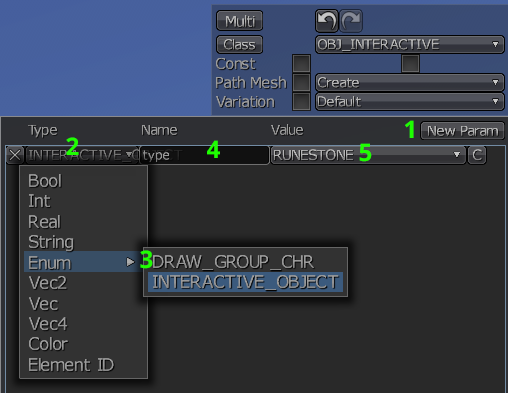
\includegraphics[width=0.8\linewidth]{images/objClassParams.png}
\caption[]{Custom Parameters for an object class.}
\label{fig:objClassParams}
\end{figure}	

Je hebt nu een parameter toegevoegd aan je object class. In dit geval was dat een enumeratie, maar je ziet dat je eender welke variabele kan maken. In je code heb je toegang tot deze waarden, dus je kan ze gebruiken om het gedrag van je object aan te passen.

\begin{exercise}
	\begin{enumerate}
		\item Open Assets $\Rightarrow$ other $\Rightarrow$ runestone en kies de tab `Params'. De parameter type werd overgenomen van de object class.
		\item Voeg nog een parameter toe aan je runestone. Deze keer kies je het type `Int', Name `ID' en Value `0'.
		\item Open de world editor en kies het tabblad `Object'. Selecteer daarna een runestone.
		\item Controleer of elke runestone de gewenste parameters bevat.
		\item Pas de waarde van ID voor elke runestone aan, zodat ze de ID's van 0 tot 3 bevatten.
	\end{enumerate}
\end{exercise}

\begin{note}
Je ziet dat er een vinkje verschijnt voor een parameter wanneer je die een nieuwe waarde geeft. Daaraan zie je dat deze waarde afwijkt van de oorspronkelijke waarde. Het gebruik van parameters is ietwat gelijk aan het principe van overerving. Je kan parameters ingeven op het niveau van de object class, op het niveau van het object, of op het niveau van de instantie van het object. Elk niveau kan het vorige niveau overschrijven.

Het is ook mogelijk om alle parameters op het niveau van de instantie te schrijven. Dat betekent echter meer werk en een grotere kans op fouten.
\end{note}

\section{Retrieving Object Params in Code}

Om de object parameters in code te gebruiken, dien je de functie \eeFunc{create} van de base class \eeClass{Game.Static} te overschrijven. Daarin voer je eerst die base class functie uit. Om de parameters in code op te slaan voeg je ook twee variabelen toe. Je class ziet er nu zo uit.

\begin{code}
class interactiveObject : Game.Static
{
private:
   INTERACTIVE_OBJECT iObjType = IO_NONE;
   int ID = 0;
   
public:   
   virtual void create(Object &obj)
   {
      super.create(obj);
      
      // every interactive object has a Type parameter
      iObjType = obj.getParam("Type").asEnum();
      
      if(iObjType == IO_RUNESTONE)
      {
         // every runestone has an ID parameter
         ID = obj.getParam("ID").asInt();
      }
   }
}

Game.ObjMap<interactiveObject> InteractiveObjects;
\end{code}

Zoals je ziet heeft \eeClass{Object} een lidfunctie \eeFunc{getParam} die je toegang geeft tot de parameters. Aangezien de code niet weet welk type je parameter heeft, moet je zelf aangeven hoe je de parameter aan je code wil doorgeven. Dat kan via functies zoals \eeFunc{asEnum()} of \eeFunc{asInt()}.

\section{Particles}
Om de runestones wat meer uitstraling te geven voegen we aan elke runestone een particle effect toe. Voeg eerst de volgende variabelen toe aan de \eeClass{interactiveObject} class:

\begin{code}
Game.ObjParticles fx;
Vec fxPos;
\end{code}

Particles zijn kleine afbeeldingen waarvan je de beweging en de levensduur kan instellen. In een game worden ze vaak gebruikt om een vuur te tonen, of als visualisatie van een spell. In Esenthel is een particle een game object met als base class \eeClass{OBJ\_PARTICLE}. Wanneer je bij de parameters van een object deze base class instelt, krijg je automatisch toegang tot alle parameters van een particle.

\begin{note}
De object class \eeClass{OBJ\_PARTICLE} moet dan wel al die parameters bevatten. Als je aan een eigen project werkt, dan kan je deze class best copi\"eren van een voorbeeldproject. 
\end{note}

Het oefenproject bij dit hoofdstuk bevat al een uitgewerkte particle in Assets$\Rightarrow$other$\Rightarrow$runestone$\Rightarrow$particle. We zullen deze particle in het object fx laden. Voor we dat doen zullen we eerst een geschikte positie moeten vinden. Het is de bedoeling dat de particles zichtbaar zijn in de holle opening van de runestone. 

Met die reden is aan het runestone object een `slot' toegevoegd. Je kan dat nakijken door het object in de editor te openen en de tab `slots' te kiezen. Selecteer de optie om een positie aan te passen en hover over het aanwezige slot. Je zal zien dat dit slot een naam heeft: `particle'. Via deze naam kunnen we de positie van het slot opvragen. Aangezien we in de world editor ook elke runestone een andere schaal zouden kunnen geven, is het belangrijk dat deze positie geschaald wordt.

Ook belangrijk om te onthouden is dat het om een relatieve positie gaat. Het slot heeft geen positie in de wereld, maar een offset ten opzichte van de positie van de runestone. In dit geval komt dat goed uit. We geven fx ook de positie van de runestone, maar de bron van de particles moet relatief zijn ten opzichte van die positie. Als bron stellen we een \eeClass{Ball} in die de positie van het slot krijgt.

De volledige create functie ziet er dan zo uit:
\begin{code}
virtual void create(Object &obj)
{
  super.create(obj);
  
  iObjType = (INTERACTIVE_OBJECT)obj.getParam("Type").asEnum(); 
  if(iObjType == IO_RUNESTONE)
  {
     ID = obj.getParam("ID").asInt();
     
     if(mesh->skeleton().findPoint(8"particle") != null)
     {
        fxPos = mesh->skeleton().findPoint(8"particle").pos * scale;
        fx.create(*Objects(=== drop particle object here ===));
        fx.pos(pos());
        fx.particles.source(Ball(0.1, fxPos));
     } 
  }
}
\end{code}

\begin{exercise}
Voeg deze code toe aan je project.
\end{exercise}

Particles zijn bewegende afbeeldingen en moeten ook geupdated worden. Daarvoor heeft de class \eeClass{Game.ObjParticles} een update functie. Het volstaat om deze functie uit te voeren. Maar omdat de \eeClass{interactiveObject} class niet enkel voor runestones dient, doen we dit enkel wanneer \eeClass{iObjType} een runestone is:

\begin{code}
virtual Bool update()
{
  if(iObjType == IO_RUNESTONE)
  {
     // update the particles
     fx.update();
  }
  
  return super.update();
}
\end{code}

Particles worden gerendered in een afzonderlijke draw functie. Afhankelijk van het soort particles heb je \'e\'en van de volgende render modes nodig:

\begin{itemize}
	\item RM\_BLEND
	\item RM\_PALETTE
	\item RM\_PALETTE1
\end{itemize}

In de \eeFunc{drawPrepare} functie moet je daarom de gewenste render mode toevoegen. In dit geval gebruiken we RM\_PALETTE.

\begin{code}
virtual UInt drawPrepare()
{     
  uint result = super.drawPrepare();  
  if(iObjType == IO_RUNESTONE)
  {
     result |= IndexToFlag(RM_PALETTE);
  } 
  return result;
}
\end{code}

Tot slot moet je ook de functie \eeFunc{drawPalette} overschrijven:
\begin{code}
virtual void drawPalette()
{
   fx.drawPalette();
}
\end{code}

\begin{exercise} 
Voeg alle bovenstaande code toe aan je project. Voer je game uit en controleer of je de particles op het scherm ziet.
\end{exercise}

\section{Licht}
Een andere techniek die de game wat meer sfeer kan geven is het toevoegen van lichtbronnen. Hier moet je wel voorzichtig mee omgaan. Voor elke lichtbron moeten immers ook schaduwen berekend worden. Een scene met veel lichtbronnen kan bijzonder zwaar zijn voor een oudere computer. Ook mobile games zijn meestal beperkt tot \'e\'en enkele bron.

Een lichtbron toevoegen is alvast heel eenvoudig. Je hebt enkel een positie en een kleur nodig. (Al zijn er extra argumenten om ook de intensiteit en de maximum afstand te bepalen, maar hier gebruik je de defaults.)

Je voegt deze code toe aan de \eeFunc{drawPrepare} functie:
\begin{code}
if(iObjType == IO_RUNESTONE)
{
   LightPoint(1, pos() + fxPos, GREEN.asVec()).add();
   result |= IndexToFlag(RM_PALETTE);
}
\end{code}

\begin{exercise}
Experimenteer met de instellingen van de lichtbron. Wijzig ook de parameters van het particle object, zodat je een beter zicht krijgt op de betekenis van de parameters.
\end{exercise}

\section{Toggle the Runes}
Op dit moment zijn de particles en het licht steeds actief. Nu ga je er voor zorgen dat je ze in en uit kan schakelen door er op te klikken. Een groot deel van deze code ken je al uit de vorige secties. Zo zullen we eerst een outline toevoegen wanneer je muis over een runestone hovert.

\begin{enumerate}
	\item Voeg eerst deze variabelen toe aan de \eeClass{interactiveObject} class:

\begin{code}
bool belowMouse = false;
bool active = false;
\end{code}
	\item In de \eeFunc{update} functie zorg je er voor dat \eeFunc{belowMouse} steeds false wordt.
	\item Je voegt daarna de outline render mode toe in \eeFunc{drawPrepare}, maar enkel waneer \eeFunc{belowMouse} de waarde true heeft.
	\item zorg er ook voor dat het \eeClass{LightPoint} en de particles enkel getoond worden wanneer `active' true is.
	\item Nu overschrijf je de \eeFunc{drawOutline} functie. Als je niet zeker bent, kan je spieken in de \eeClass{magicLamp} class.
	\item Tot slot voeg je enkele eenvoudige functies toe die je later van pas zullen komen. Je ziet hieronder de declaraties. Je kan deze functies (telkens precies \'e\'en statement) zeker zelf uitwerken.

\begin{code}
   bool isRuneStone   () { ???; }  
   void setBelowMouse () { ???; }  
   void toggleActive  () { ???; }
   void deactivate    () { ???; }
   bool isActive      () { ???; } 
   int  getID         () { ???; }   
   Vec  getParticlePos() { ???; }
\end{code}

\end{enumerate}

In de class \eeClass{inputControl} kan je nu een extra controle op de physics selector uitvoeren:

\begin{code}
if (interactiveObject  * obj = CAST(interactiveObject, selector.obj))
{
	if(obj.isRuneStone())
	{
	   obj.setBelowMouse();
	   if(Ms.bp(0))
	   {
	      obj.toggleActive();
	   }
	}
}
\end{code}

\begin{exercise}
Wanneer je alle code toegevoegd hebt, voer je de game uit en controleer je of alles werkt.
\end{exercise}


\section{A Puzzle}
In het laatste deel van dit hoofdstuk maak je een puzzel. Het is de bedoeling de 4 runestones in de juiste volgorde activeert. Als ze alle vier actief zijn, komt het hoofd in het midden naar boven. Ook toon je een laser effect tussen de actieve runestones. Je start met een nieuwe class \eeClass{puzzle}:

\begin{code}
class puzzle {
private:
	Mems<interactiveObject *> objects;
	Mems<Vec> laserPoints;
	Sound sound;

public:

}
puzzle Puzzle;
\end{code}

De \eeClass{objects} container bevat pointers naar de aanwezige runestones in de game wereld. \eeClass{laserPoints} zal de punten bevatten waartussen en laser getoond moet worden. En tot slot is er een \eeClass{sound} om alles wat spannender te maken.

Je voegt nu in het private deel van de class de volgende functies toe:

\begin{code}
interactiveObject * getObjectWithID(int ID)
{
  REPA(objects)
  {
     if(objects[i].getID() == ID) return objects[i];
  }
  
  return null;
}

void turnOffStones()
{
  REPA(objects) objects[i].deactivate();
}
\end{code}

Deze functies maken de volgende code eenvoudiger:

\begin{description}
	\item[getObjectWithID] zoek de runestone met het gevraagde ID. De volgorde in de container is immers niet gelijk aan de volgorde van de ID's.
	\item[turnOffStones] deactiveert alle runestones in de container.
\end{description}

De volgende functies die je aanmaakt zorgen er voor dat je runestones kan toevoegen en verwijderen uit de container. Je moet er namelijk rekening mee houden dat Esenthel oneindig grote werelden ondersteunt. Dat betekent dat niet de hele wereld steeds in het geheugen zit. World Objects kunnen geladen en terug verwijderd worden terwijl je de speler verplaatst doorheen de game world.

\begin{code}
void registerStone(interactiveObject * obj)
{
  objects.add(obj);
}

void unregisterStone(interactiveObject * obj)
{
  REPA(objects)
  {
     if(objects[i] == obj)
     {
        objects.remove(i);
        return;
     }
  }
}
\end{code}

Nu komt het er op aan om deze functies op de juiste plaats te gebruiken. We laten elke runestone zichzelf registeren bij de puzzel. Dat kan het best in de \eeFunc{create} functie van interactiveObject. Zoek zelf even naar de meest geschikte plaats binnen deze functie en voeg de volgende code toe:

\begin{code}
Puzzle.registerStone(this);
\end{code}

Het object moet zich ook verwijderen uit de puzzel wanneer het niet langer actief is. Nu bestaat er geen functie binnen Game.Static die uitgevoerd wordt wanneer dit het geval is. Maar je kan wel kijken wat het resultaat is van update. Bij `false' zal de game engine het object verwijderen. Het komt er dus op aan om net ervoor de runestone uit de puzzel te verwijderen. Op het eind van de update functie schreven we tot hiertoe steeds:

\begin{code}
return super.update();
\end{code}

\begin{exercise}
Herschrijf de bovenstaande regel zo dat je het resultaat van \eeFunc{super.update()} kan gebruiken om het object te verwijderen als dat nodig is. 
\end{exercise}

De echte logica van de puzzel zit in de update functie. We overlopen stap voor stap wat hier moet gebeuren. Eerst wordt de container met punten voor de laser leeggemaakt. En wanneer er geen 4 runestones geladen zijn heeft het in elk geval geen zin om de puzzel te controleren.

\begin{code} 
void update() {
  laserPoints.clear();
  if(objects.elms() != 4) return;
}
\end{code}

Vervolgens controleren we de huidige stand van zaken. We kunnen er van uit gaan dat je nooit twee runestones op hetzelfde moment kan inschakelen. Daarom is het mogelijk om de volgende logica toe te passen:
\begin{enumerate}
	\item Stel de hoogst actieve ID gelijk aan nul.
	\item Ga alle runes af, beginnend met het hoogste ID.
	\item Indien dat ID actief is en de huidige hoogst actieve ID kleiner dan deze, wordt dit de hoogst actieve ID.
	\item Indien de ID kleiner is dan de hoogst actieve ID en niet actief is, dan is de puzzel ongeldig en stop je de loop.
\end{enumerate}

De code ziet er zo uit:
\begin{code}
int highestActive = 0;
bool invalid = false;
for(int i = 3; i >= 0;  i--)
{
  if(highestActive < i && getObjectWithID(i).isActive())
  {
     highestActive = i;
  } else if(highestActive > i && !getObjectWithID(i).isActive())
  {
     invalid = true;
     break;
  }
}
\end{code}

In de volgende stap zijn er twee mogelijkheden: Invalid kan true of false zijn. Wanneer de puzzel ongeldig is, dan kunnen we eenvoudigweg alle stenen uitschakelen. Dat zorgt er voor dat de speler terug opnieuw moet beginnen.

In het andere geval moet je de posities van de actieve stenen toevoegen aan de laserPoints container, maar enkel wanneer de hoogst actieve positie groter is dan 0. (Met slechts 1 actieve positie kan je toch geen lijn maken.)

Wanneer alle stenen actief zijn, dan voeg je op het eind nogmaals de eerste positie toe, zodat de `cirkel' gesloten is.

\begin{code}
if(invalid)
{
  turnOffStones();
} else if(highestActive > 0)
{
  // add points to laser
  for(int i = 0; i <= highestActive; i++)
  {
    laserPoints.add(getObjectWithID(i).getParticlePos());
  }
 
  // close trajectory if all stones are on
  if(highestActive == 3)
  {
    laserPoints.add(getObjectWithID(0).getParticlePos());
  }
}
\end{code}

Op het eind van de update functie kan je zelf code toevoegen de nodige geluiden te spelen. Je vertrekt van de volgende regels:

\begin{itemize}
	\item Wanneer laserPoints ten minste \'e\'en element bevat en \eeClass{sound} nog niet speelt, dan start je het geluid `erie\_ring' in een loop.
	\item Wanneer laserPoints leeg is en het \eeClass{sound} w\'el speelt, dan stop je het geluid met een fadeout, en je speelt het geluid `roar' (zonder loop, via de functie \eeFunc{SoundPlay}).
\end{itemize}

De laatste twee functies in deze class zijn weer eenvoudig. De \eeFunc{draw} functie toont de laser op het scherm en de \eeFunc{solved} functie laat weten of de puzzel al dan niet opgelost is.

\begin{code}
void draw()
{
  if(laserPoints.elms() > 0)
  {
     DrawLaser(GREEN, WHITE, 0.01, 0.03, false, laserPoints);
  }     
}

bool solved()
{
  return laserPoints.elms() == 5;
}
\end{code}

Omdat Puzzle geen deel uitmaakt van de Game World en toch een draw functie heeft, moet je die zelf uitvoeren. De declaratie van DrawLaser vertelt je dat er twee render modes nodig zijn: RM\_SOLID en RM\_AMBIENT. Je voegt die toe aan de \eeFunc{Render} functie in het bestand `main'.

\begin{code}
void Render()
{
   Game.World.draw();
   
   switch(Renderer())
   {
      case RM_SOLID:
      {
         Puzzle.draw();
         break;
      }
      
      case RM_AMBIENT:
      {
         Puzzle.draw();
         break;
      }
   }
}
\end{code}

Tot slot is het de bedoeling om het hoofd tussen de runes te tonen wanneer de puzzel opgelost is. Het hoofd wordt ook geladen als \eeClass{interactiveObject}, maar heeft als \eeClass{iObjType} IO\_HEAD.

Voeg eerst een variabele toe aan \eeClass{interactiveObject}.

\begin{code}
float origHeadPosY;
\end{code}

Nu kan je die oorspronkelijke Y positie van het hoofd onthouden in de \eeFunc{create} functie, om daarna het hoofd 2 units naar beneden te plaatsen:

\begin{code}
if(iObjType == IO_HEAD)
{
  origHeadPosY = pos().y;
  Vec newPos = pos();
  newPos.y -= 2;
  pos(newPos);
}
\end{code}

Daarna kan je in de update functie het hoofd verplaatsen wanneer nodig:

\begin{code}
if(iObjType == IO_HEAD)
{
  if(Puzzle.solved() && pos().y < origHeadPosY)
  {
     your code here!
  }
  else if(!Puzzle.solved() && pos().y > origHeadPosY - 2)
  {
	 .. and here!
  }
}
\end{code}

\begin{exercise}
Vul de bovenstaande code verder aan en test of alles werkt.
\end{exercise}
